\chapter{Sequences in Calculus}

We have introduced sequences in a previous chapter. Now, we will examine them in more detail in a calculus context. You already know about arithmetic and geometric sequences, but not all sequences can be classified as arithmetic or geometric. Take the famous Fibonacci sequence, \{1, 1, 2, 3, 5, 8, ...\}, which can be explicitly defined as $a_n = a_{n-1} + a_{n-2}$, with $a_1 = a_2 = 1$. There is no common difference or common ratio, so the Fibonacci sequence is not arithmetic or geometric. Another example is $a_n = \sin{\frac{n\pi}{6}}$, which will cycle through a set of values. In later chapters, you will learn that the sum of all the values in a sequence is a series and how to use series to describe functions. In order to be able to do all that, first we need to talk in-depth about sequences. 

Some sequences are defined explicitly, like $a_n = \sin{\frac{n\pi}{6}}$, while others are defined recursively, like $a_n = a_{n-1} + a_{n-2}$. 

Example: Write the first 5 terms for the explicitly defined sequence $a_n = \frac{n}{n+1}$.

Solution: We can construct a table to keep track of our work:
\begin{center}
\begin{tabular}{|c|c|c|}\hline
$n$ & work & $a_n$\\
\hline
1 & $\frac{1}{1+1}$ & $\frac{1}{2}$\\
\hline
2 & $\frac{2}{2+1}$ & $\frac{2}{3}$\\
\hline
3 & $\frac{3}{3+1}$ & $\frac{3}{4}$\\
\hline
4 & $\frac{4}{4+1}$ & $\frac{4}{5}$\\
\hline
5 & $\frac{5}{5+1}$ & $\frac{5}{6}$\\
\hline
\end{tabular}
\end{center}

\begin{Exercise}[label = seqcalc1]
Write the first 5 terms for each sequence. 
\begin{enumerate}
\item $a_n = \frac{2^n}{2n+1}$
\item $a_n = \cos{\frac{n\pi}{2}}$
\item $a_1 = 1$, $a_{n+1} = 5a_n-3$
\item $a_1 = 6$, $a_{n+1} = \frac{a_n}{n+1}$
\end{enumerate}
\end{Exercise}

\begin{Answer}[ref=seqcalc1]
\begin{enumerate}
\item $\frac{2}{3}$, $\frac{4}{5}$, $\frac{8}{7}$, $\frac{16}{9}$, 
$\frac{32}{11}$
\item 0, -1, 0, 1, 0
\item 1, 2, 7, 32, 157
\item 6, 3, 1, $\frac{1}{4}$, $\frac{1}{20}$
\end{enumerate}
\end{Answer}

%fibanocci and [(-1)^(n-1)]/n as examples of sequences that are not strictly arithmetic or geometric

%exercise - list fist 5 terms of more complex sequences
%exercise - find explicit formulas seqcalc2

%define convergent and divergent sequence
You can visualize a sequence on an $xy$-plane or a number line. 
Figures \ref{fig:linefrac} and \ref{fig:planefrac} show visualizations 
of the sequence $a_n = \frac{n}{n+1}$. To visualize this on the 
$xy$-plane, we take points such that $x = n$ and $y = a_n$, where $n$ 
is a positive integer. What do you notice about this sequence? As $n$ 
increases, $a_n$ gets closer and closer to $1$. 

\begin{figure}[htbp]
\centering
    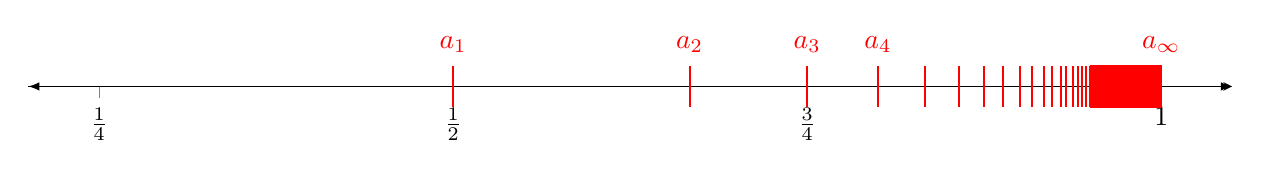
\begin{tikzpicture}
        \begin{axis}[axis y line = none, width = 2*\axisdefaultwidth, 
        height = 0.25*\axisdefaultwidth, axis lines = center, 
        xtick align = outside, xmin = 0.2, xmax = 1.05, 
        xtick = {0.25, 0.5, 0.75, 1}, xticklabels = {$\frac{1}{4}$, 
        $\frac{1}{2}$, $\frac{3}{4}$, $1$}, ymin = -0.5, ymax = 0.5, 
        clip = false]
        \draw[latex-latex](0.2, 0) --(1.05,0);
        \draw[red, thick] (0.5, -0.5) -- (0.5, 0.5);
        \draw[red, thick] (0.667, -0.5) -- (0.667, 0.5);
        \draw[red, thick] (0.75, -0.5) -- (0.75, 0.5);
        \draw[red, thick] (0.8, -0.5) -- (0.8, 0.5);
        \draw[red, thick] (0.833, -0.5) -- (0.833, 0.5);
        \draw[red, thick] (0.857, -0.5) -- (0.857, 0.5);
        \draw[red, thick] (0.875, -0.5) -- (0.875, 0.5);
        \draw[red, thick] (0.888, -0.5) -- (0.888, 0.5);
        \draw[red, thick] (0.9, -0.5) -- (0.9, 0.5);
        \draw[red, thick] (0.909, -0.5) -- (0.909, 0.5);
        \draw[red, thick] (0.917, -0.5) -- (0.917, 0.5);
        \draw[red, thick] (0.923, -0.5) -- (0.923, 0.5);
        \draw[red, thick] (0.929, -0.5) -- (0.929, 0.5);
        \draw[red, thick] (0.933, -0.5) -- (0.933, 0.5);
        \draw[red, thick] (0.9375, -0.5) -- (0.9375, 0.5);
        \draw[red, thick] (0.941, -0.5) -- (0.941, 0.5);
        \draw[red, thick] (0.944, -0.5) -- (0.944, 0.5);
        \draw[red, thick] (0.947, -0.5) -- (0.947, 0.5);
        \draw[red, thick] (0.95, -0.5) -- (0.95, 0.5);
        \filldraw[red](0.95, -0.5) rectangle (1, 0.5);
        \node[red] at (0.5, 1) {$a_1$};
        \node[red] at (0.667, 1) {$a_2$};
        \node[red] at (0.75, 1) {$a_3$};
        \node[red] at (0.8, 1) {$a_4$};
        \node[red] at (1, 1) {$a_{\infty}$};
        \end{axis}
\end{tikzpicture}
    \caption{$a_n =\frac{n}{n+1}$ on a number line}
    \label{fig:linefrac}
\end{figure}

\begin{figure}[htbp]
\centering
    \begin{tikzpicture}
        \begin{axis}[axis lines = center, xmin = -0.5, xmax = 15, 
        ymin = -0.5, ymax = 1.5, xlabel=$n$, ylabel = $a_n$]
        \addplot[blue, dashed] coordinates {(0, 1) (15, 1)};
        \addplot[mark=*, red] (1, 0.5);
        \addplot[mark=*, red] (2, 0.667);
        \addplot[mark=*, red] (3, 0.75);
        \addplot[mark=*, red] (4, 0.8);
        \addplot[mark=*, red] (5, 0.833);
        \addplot[mark=*, red] (6, 0.857);
        \addplot[mark=*, red] (7, 0.875);
        \addplot[mark=*, red] (8, 0.888);
        \addplot[mark=*, red] (9, 0.9);
        \addplot[mark=*, red] (10, 0.909);
        \addplot[mark=*, red] (11, 0.917);
        \addplot[mark=*, red] (12, 0.923);
        \addplot[mark=*, red] (13, 0.929);
        \addplot[mark=*, red] (14, 0.933);
        \addplot[mark=*, red] (15, 0.9375);
        \end{axis}
\end{tikzpicture}
    \caption{$a_n =\frac{n}{n+1}$ on an $xy$-plane}
    \label{fig:planefrac}
\end{figure}

Because $a_n$ approaches a specific number as $n \to \infty$, we call 
the series $a_n = \frac{n}{n+1}$ \textit{convergent}. We prove a 
sequence is convergent by taking the limit as $n$ approaches 
$\infty$. If the limit exists and approaches a specific number, the 
sequence is convergent. If the limit does not exist or approaches 
$\pm\infty$, the sequence is divergent. 

We can see graphically that $\lim_{n \to \infty} \frac{n}{n+1} = 1$, 
so that sequence is convergent. What about $b_n = \frac{n}{\sqrt{10 + 
n}}$? Is $b_n$ convergent or divergent? 
$$\lim_{n \to \infty} \frac{n}{\sqrt{10 + n}} = 
\lim_{n \to \infty} \frac{n/n}{\sqrt{\frac{10}{n^2}+ \frac{n}{n^2}}}$$
$$=\lim_{n \to \infty} \frac{1}{\sqrt{\frac{10}{n^2}+\frac{1}{n}}} = \infty$$

Therefore, the sequence $b_n = \frac{n}{\sqrt{10 + n}}$ is divergent. 

Here is another example of a divergent sequence: $c_n = 
\sin{\frac{n\pi}{2}}$. The graph is shown in figure \ref{fig:sineseq}. 
As you can see, the value of $c_n$ oscillates between 1, 0, and -1 
without approaching a specific number. This means that $c_n$ does 
not approach a particular number as $n \to \infty$ and the sequence is 
divergent. 

\begin{figure}[htbp]
\centering
    \begin{tikzpicture}
        \begin{axis}[axis lines = center, xmin = -0.5, xmax = 8, 
        ymin = -1.5, ymax = 1.5, xlabel=$n$, ylabel = $c_n$]
        \addplot[mark=*, red] (1, 1);
        \addplot[mark=*, red] (2, 0);
        \addplot[mark=*, red] (3, -1);
        \addplot[mark=*, red] (4, 0);
        \addplot[mark=*, red] (5, 1);
        \addplot[mark=*, red] (6, 0);
        \addplot[mark=*, red] (7, -1);
        \addplot[mark=*, red] (8, 0);
        \end{axis}
\end{tikzpicture}
    \caption{$c_n =\sin{\frac{n\pi}{2}}$ on an $xy$-plane}
    \label{fig:sineseq}
\end{figure}

%exercise - classify sequences as convergent or divergent
\begin{Exercise}[label=seqcalc3]
Classify each sequence as convergent or divergent. If the sequence is 
convergent, find the limit as $n \to \infty$.
\begin{enumerate}
\item $a_n = \frac{3 + 5n^2}{n + n^2}$
\item $a_n = \frac{n^4}{n^3 - 2n}$
\item $a_n = 2 + (0.86)^n$
\item $a_n = \cos{\frac{n\pi}{n+1}}$
\item $a_n = \sin{n}$
\end{enumerate}
\end{Exercise}

\begin{Answer}[ref=seqcalc3]
\begin{enumerate}
\item convergent, 5
\item divergent
\item convergent, 2
\item convergent, -1
\item divergent
\end{enumerate}
\end{Answer}

%define increasing, decreasing, monotonic, and bounded sequences